\graphicspath{{./Introduccion/Figures/}}

La caracter\'istica principal de los semiconductores es la separaci\'on o gap entre la banda de valencia y la banda de conducci\'on, con un valor pequeño ($\varepsilon_g  = \varepsilon_C - \varepsilon_V \sim 0.1 - 3$ eV). Al tener un gap pequeño pueden darse saltos entre electrones de la banda de valencia y la banda de conducci\'on, apartir de la mediaci\'on de un fot\'on. Estas interacciones solo se pueden dar para energias del fot\'on $h\nu > \varepsilon_g$.

Las tres posibles formas de interacci\'on luz-materia son la emisi\'on espont\'anea, la emisi\'on estimulada y la absorci\'on. En un material semiconductor a $T = 0$K se tiene la banda de valencia completamente llena y la banda de conducci\'on vac\'ia. Al aumentar la temperatura se pueden dar saltos de los electrones a la banda de conducci\'on debido al pequeño gap. Al situarse un electr\'on en un nivel superior de energ\'ia, \'este tender\'a a volver a su estado de m\'inima energ\'ia recombinandose de nuevo en la banda de valencia, pudiendo emitir un fot\'on en el proceso. Este proceso es el denominado emisi\'on espont\'anea en el que cada fot\'on puede tener diferente fase y direcci\'on.

	\begin{figure}[H]
		\centering
		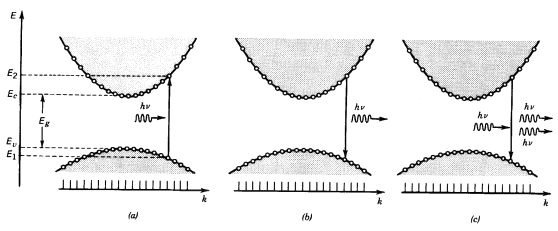
\includegraphics[width=0.6\linewidth]{BV-BC.png}
		\caption{\label{Img:Saleh-BV-BC}Esquema de bandas con las tres interacciones luz-materia en un semiconductor: (a) absorci\'on, (b) emisi\'on espont\'anea y (c) emisi\'on estimulada \cite{saleh2019fundamentals}.}
	\end{figure}

El proceso clave para los l\'aseres de semiconductor, al igual que para el resto, es la emisi\'on estimulada. Si sobre el material con un electr\'on excitado en la banda de conducci\'on, se incide con un fot\'on de frecuencia $\nu_0$ igual a la diferencia de energ\'ias entre el estado excitado del electr\'on y el fundamental, existe una probabilidad mayor de que el electr\'on decaiga al nivel de menor energ\'ia. El fot\'on emitido en la recombinaci\'on del electr\'on tendr\'a las mismas propiedades que el fot\'on incidente, pudiendo estos dos fotones interactuar con m\'as electrones excitados y as\'i producir la amplificaci\'on de la radiaci\'on incidente. Sin embargo, para que esta amplificaci\'on continue, debe haber una cantidad suficiente de electrones excitados. Para ello se utilizan fuentes de bombeo para obtener la inversi\'on de poblaci\'on.

El medio en el cu\'al se producen la mayor parte de emisiones espont\'aneas y estimuladas se denomina medio activo y para los l\'aseres de semiconductor suelen ser heteroestructuras por capas con una uni\'on $pn$ en la direcci\'on de avance de la corriente. Cuando la corriente inyectada al l\'aser es suficientemente grande, se obtienen suficientes electrones en la banda de conducci\'on para amplificar la luz. Una ventaja de los l\'aseres de semiconductor es su alta densidad de electrones, que permiten alcanzar grandes valores para la ganancia y unas distancias pequeñas de la cavidad, del orden de $\sim 1$ mm.

La direcci\'on del medio activo con respecto al haz de luz emitido permite diferenciar entre dos tipos de l\'aseres de semiconductor. Los l\'aseres de emisi\'on vertical (VCSEL) presentan el medio activo ortogonal al haz de luz mientras que para los de emisión lateral el medio activo es paralelo al haz de luz emitida. 

El tipo de l\'aser de semiconductor que consideraremos en este trabajo es un l\'aser de emisi\'on lateral que emite en un solo modo y se llama l\'aser de modo discreto (DML). Este tipo de l\'aser se caracteriza por perturbaciones en el indice de refracci\'on debidas a unos surcos paralelos a la regi\'on activa debajo del contacto el\'ectrico y realizados durante la fabricaci\'on, que seleccionan un \'unico modo longitudinal.
